\documentclass[journal]{IEEEtran}

\usepackage{amsmath}
\usepackage{graphicx}
\usepackage{algorithm}
\usepackage{algorithmic}
\usepackage{url}
\usepackage{tikz}
\usetikzlibrary{shapes.geometric, arrows, positioning}

\title{Design and Implementation of an Autonomous Search and Rescue Robot in Webots}

\author{
    \IEEEauthorblockN{Patrick, Junlin, Hana, and Maureen} \\
    \IEEEauthorblockA{School of Computer Science, University of Birmingham}
}

\begin{document}

\maketitle

\begin{abstract}
This report outlines the development of an autonomous search and rescue robot using the Webots simulation environment. The system is engineered to navigate known environments populated with unknown obstacles to locate victims. The control architecture is governed by a Finite State Machine that orchestrates four distinct modules: Path Planning, Navigation, Victim Detection, and Localisation.

The path planning module utilises the $A^*$ algorithm to generate optimal paths for either targeted inspection of specific locations or complete area coverage. Navigation combines global path following with reactive obstacle avoidance to handle unknown hazards. Victim identification uses a stop-and-scan method, integrating colour-based vision and depth sensing to localise targets relative to the robot's position. Experimental validation in a simulated environment confirmed the system's ability to maintain effective coverage while successfully identifying and locating victims and avoiding collisions.
\end{abstract}

\section{Introduction}

The deployment of autonomous robotic systems in post-disaster scenarios offers a critical advantage in minimising risk to human responders while accelerating the detection of survivors. However, environments struck by disaster present a unique navigational challenge: while the general structural layout (e.g., walls, rooms) may be known from prior blueprints, the traversal of the area is often compromised by unpredictable debris and rubble.

This project addresses this challenge by developing a control architecture for a Pioneer 3-DX robot within the Webots simulation environment \cite{michel2004cyberbotics}. The primary objective is to achieve autonomous coverage of a specified search area to identify and locate victims. To accomplish this, we implemented a modular Finite State Machine that coordinates four distinct modules: Path Planning, Navigation, Victim Detection, and Localisation. This framework allows the robot to switch seamlessly between systematic area coverage, reactive obstacle avoidance, and high-precision visual scanning.

This report details the design and real-time integration of the proposed system. Section II reviews the foundational algorithms ($A^*$, APF, HSV Colour Segmentation); Section III describes the simulation environment and robot configuration; Section IV details the algorithmic implementation of the control architecture; and Section V presents the experimental evaluation of the system's efficiency and robustness in cluttered topologies.

\section{Related Work}

This project integrates standard, well-established algorithms in robotics. For global path planning, we rely on the $A^*$ algorithm introduced by Hart et al. \cite{hart1968formal}, which is the industry standard for optimal pathfinding in static grid maps. To handle dynamic navigation, we utilise the Artificial Potential Field (APF) method proposed by Khatib \cite{khatib1986real}, which allows for reactive obstacle avoidance. Finally, for victim identification, we employ standard colour-based computer vision techniques utilising the HSV colour space, implemented via the OpenCV library \cite{bradski2000opencv}.

Beyond individual planning and avoidance techniques, the integration of global path planning with LiDAR-based local obstacle avoidance has also been widely studied in mobile robotics. A common architectural assumption is that a global planner provides long-term navigation guidance, while a local reactive layer, driven by LiDAR sensing, handles short-range obstacle avoidance and allows the robot to temporarily deviate from the planned path when necessary. Once the obstacle is cleared, the robot is expected to rejoin the original global route.

However, prior studies have shown that this integration is non-trivial in practice. Purely reactive LiDAR-based avoidance strategies do not inherently preserve global path consistency, particularly in cluttered or dynamic environments. Without explicit replanning, state recovery, or tight coupling between planning and perception modules, repeated local corrections may cause the robot to drift away from the intended trajectory, leading to oscillatory behaviour or navigation failure. These challenges motivate further investigation into the interaction between global planning and local avoidance mechanisms under realistic sensing and computational constraints.


\section{System Setup and Problem Definition [Patrick]}

\subsection{Simulation Environment and Robot}
The system is developed within the Webots simulation platform, utilising a Pioneer 3-DX mobile robot. The robot is equipped with a SICK LMS-291 LIDAR on the front of the robot for distance measurement and a forward-facing RGB camera placed on top of the robot.

The continuous known environment is mapped onto a binary occupancy grid with 0 representing an available cell and 1 representing a cell that is occupied by a known obstacle. This grid is defined as a two-dimensional list where each internal list represents a row. The default configuration utilises a cell size of 1.0m x 1.0m, though this parameter is adjustable to allow for a higher-resolution simulated environment if required. The obstacles are implemented as 0.8m cubes with a brick texture applied.

\subsection{Victim Definition}
Victims are represented within the simulation as static, green 0.35m cubes. This colour choice was selected to maximise segmentation contrast against the environment's floor and wall textures.

\section{Algorithms and Framework}
% ============================
% Added LiDAR exploration section (Junlin Lu)
% ============================
\subsection{LiDAR Integration and Design Exploration [Junlin Lu]}

During system development, an exploratory implementation was conducted to investigate the integration of LiDAR-based local obstacle avoidance with the global path planning framework. The LiDAR sensor was successfully activated and configured to provide real-time range measurements, which were continuously monitored through console output during robot execution. This confirmed correct sensor operation and data availability for reactive control.

The LiDAR integration and avoidance logic were initially implemented and validated within an early 5$\times$5 experimental robot setup. To support this functionality, modifications were required in both the main control program and the local obstacle avoidance submodule. Within this simplified environment, real-time LiDAR feedback was successfully used to detect nearby obstacles and generate avoidance-related diagnostic outputs, demonstrating the feasibility of LiDAR-driven reactive behaviour at the subsystem level.

When attempting to integrate the modified main controller into the updated project structure and larger navigation map, compatibility issues were encountered. These issues were primarily related to differences in map representation, control flow assumptions, and module interfaces between the initial experimental setup and the final system architecture. Due to limited remaining development time, a full reintegration and debugging process within the updated GitHub Webots project could not be completed.

As a result, this LiDAR-based exploration is presented as a validated design experiment rather than a fully integrated component of the final system. A supplementary demonstration video is provided to illustrate successful LiDAR activation and real-time obstacle feedback within the 5$\times$5 setup. This exploration highlights the practical challenges of combining global path planning with reactive LiDAR-based avoidance under constrained development conditions, and motivates tighter integration strategies in future work.



\subsection{System Architecture and Driver Code [Patrick]}
The system's core logic is encapsulated in a main module which acts as the orchestrator for all sub-modules (path planning, obstacle avoidance, localisation, and victim detection).

\subsubsection{Initialisation}
The main module is responsible for the initialisation of important configuration variables (for example, ANALYSE\_AT\_EVERY\_CELL - a boolean which determines whether or not the robot performs victim detection at every cell it visits or only at locations of interest), the definition of the occupancy grid, along with start position and locations of interest, the definition of a Finite State Machine (detailed below) and the execution of the main control loop. The main module also includes a movement class, which is utilised in the main control loop, to provide basic movement functions that enable the robot to traverse along the planned path. This movement class abstracts over Webots' controller module, providing an easy to use interface.

\subsubsection{Finite State Machine}
The main execution loop implements a Finite State Machine that governs the robot's high-level behaviour. As illustrated in the state transition logic, the system cycles through four phases:
\begin{enumerate}
    \item \textbf{INIT\_PLANNING:} The driver triggers the path planning module to generate a coordinate queue based on the initialised grid.
    \item \textbf{NAVIGATING:} The driver computes the required wheel velocities to traverse to the next waypoint.
    \item \textbf{SCANNING:} The driver halts the movement of the robot and triggers the victim detection implementation.
    \item \textbf{MISSION\_COMPLETE:} The control loop terminates, the list of victim locations is output and a function is called to generate a text-based visualization of the mission history.
\end{enumerate}

\begin{figure}[!ht]
\centering
\resizebox{\columnwidth}{!}{%
    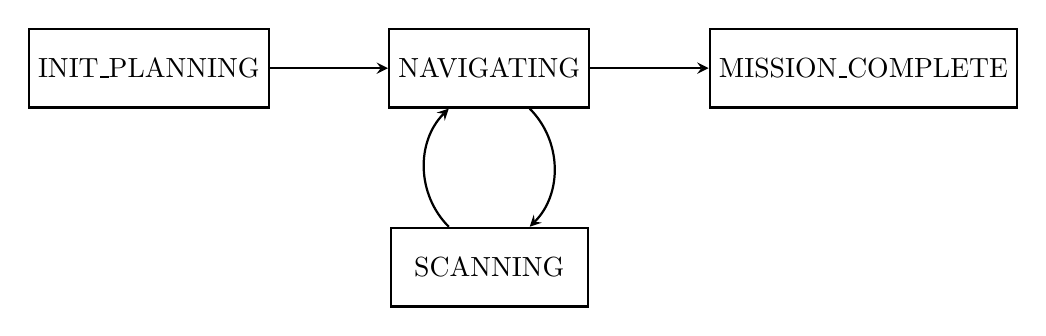
\begin{tikzpicture}[
        >=stealth,
        node distance=1.5cm,
        state/.style={rectangle, draw, thick, minimum width=2.5cm, minimum height=1cm, align=center}
    ]

    \node (init) [state] {INIT\_PLANNING};
    \node (nav) [state, right=of init] {NAVIGATING};
    \node (scan) [state, below=of nav] {SCANNING};
    \node (done) [state, right=of nav] {MISSION\_COMPLETE};

    \draw [->, thick] (init) -- (nav);
    \draw [->, thick, bend left=45] (nav) to (scan);
    \draw [->, thick, bend left=45] (scan) to (nav);
    \draw [->, thick] (nav) -- (done);

    \end{tikzpicture}
}
\caption{Finite State Machine control logic.}
\end{figure}

\subsection{Path Planning [Patrick]}
The path planning module is responsible for generating a collision-free, optimal trajectory that links all target locations. As detailed in Algorithm 1, the system constructs a global route by treating the mission as a sequential set of point-to-point navigation tasks.

\subsubsection{Route Construction Strategy}
The planner first establishes an ordered list of high-level targets. If specific Locations of Interest (LOIs) are provided, the route is constructed as a tour: $Route = [Start, LOI_1, \dots, LOI_n, Start]$. In the absence of specific targets, a helper function generates a Boustrophedon (lawnmower) pattern to cover all accessible free space.

\subsubsection{Optimal Pathfinding ($A^*$)}
To navigate between consecutive high-level waypoints (e.g., from $LOI_k$ to $LOI_{k+1}$), the system employs the $A^*$ search algorithm. This ensures that even if a straight line is blocked by walls, the robot finds the shortest valid route around them.
The algorithm maintains a priority queue of open nodes, ordered by the cost function $f(n) = g(n) + h(n)$, where:
\begin{itemize}
    \item $g(n)$ is the accumulated cost from the start node.
    \item $h(n)$ is the heuristic estimate to the goal.
\end{itemize}
Given the grid-based topology where movement is restricted to 4-connected neighbours (up, down, left, right), we utilise the Manhattan Distance as the admissible heuristic:
\begin{equation}
h(n) = |x_{current} - x_{goal}| + |y_{current} - y_{goal}|
\end{equation}

\subsubsection{Waypoint Validation}
To bridge the discrete grid logic with the continuous world, the planner implements a proximity check. A waypoint is considered ``reached'' when the robot's Euclidean distance to the target's world coordinate is less than a defined threshold ($D_{thresh} = 0.1\text{m}$). This tolerance allows for smooth path following without requiring perfect floating-point alignment.

\begin{algorithm}
\caption{Global Route Construction}
\begin{algorithmic}[1]
\REQUIRE $Grid$, $Start$, $LOIs$
\IF{$LOIs$ is empty}
    \STATE $LOIs \leftarrow \textbf{GenerateLawnmowerPattern}(Grid)$
\ENDIF
\STATE $Route \leftarrow [Start] + LOIs + [Start]$
\STATE $FullPath \leftarrow \textbf{List}()$
\FOR{$i = 0$ to $length(Route) - 1$}
    \STATE $Segment \leftarrow \textbf{A\_Star}(Route[i], Route[i+1])$
    \IF{$Segment$ is $None$}
        \STATE \textbf{Error}: Path blocked
    \ELSE
        \STATE Append $Segment$ to $FullPath$
    \ENDIF
\ENDFOR
\RETURN $FullPath$
\end{algorithmic}
\end{algorithm}

\subsection{Navigation and Control [Patrick]}
While the path planner operates in the discrete domain of grid cells, the robot requires continuous actuation signals. The Navigation module, embedded within the main driver loop, acts as a bridge between these two domains.

\subsubsection{Motion Control Logic}
The system employs a proportional controller to steer the robot towards the active waypoint. At each time step, the driver calculates the heading error $\theta_{err}$ between the robot's current orientation and the target coordinate.
The control law governs the differential wheel velocities ($v_{left}, v_{right}$) as follows:
\begin{equation}
v_{left} = V_{base} - (K_{turn} \cdot \theta_{err})
\end{equation}
\begin{equation}
v_{right} = V_{base} + (K_{turn} \cdot \theta_{err})
\end{equation}
where $K_{turn} = 2.6$ is the empirically tuned proportional gain. To prevent instability during sharp turns, the base velocity $V_{base}$ is dynamically throttled based on the severity of the turn:
\begin{equation}
V_{base} = \frac{V_{max}}{1 + |K_{turn} \cdot \theta_{err}|}
\end{equation}
This throttling mechanism ensures the robot naturally slows down when correcting large orientation errors, improving trajectory accuracy.

\subsection{Obstacle Avoidance [Junlin]}

This module provides reactive safety using Artificial Potential Fields (APF) \cite{khatib1986real}, in which obstacles are modelled as repulsive potentials that influence the robot’s motion in real time. The primary role of this module is to prevent imminent collisions by generating short-range corrective control actions based on onboard sensor feedback.

During development, the obstacle avoidance logic was explored in conjunction with LiDAR sensing to assess its effectiveness when integrated with the global path planning framework. The LiDAR sensor was successfully activated and configured to provide real-time range measurements, which were continuously monitored through console output during execution. This enabled the detection of nearby obstacles and the triggering of avoidance-related responses at runtime.

Experimental testing revealed that while APF-based avoidance is effective for immediate collision prevention, purely reactive control does not inherently preserve consistency with the globally planned path. In cluttered environments, repeated local corrections driven by LiDAR measurements may cause the robot to deviate significantly from the original trajectory. Without explicit replanning or state recovery mechanisms, such deviations can accumulate, making it difficult for the robot to reliably rejoin the intended route.

These observations highlight a fundamental limitation of reactive obstacle avoidance when used in isolation. Although APF provides a lightweight and computationally efficient solution for local safety, its integration with global navigation requires careful coordination. This motivates the need for tighter coupling between global planning and local avoidance, such as incorporating online replanning, path correction strategies, or predictive control methods in future system iterations.



\subsection{Victim Detection and Localisation [Patrick \& Hana]}
The victim detection module executes a discrete "stop-and-scan" manoeuvre. The robot rotates in place (velocity $\pm 2.3$ rad/s) for a full revolution, processing the camera feed to identify green contours in HSV space.

\subsubsection{Sensor Fusion and Alignment}
To ensure accurate geo-referencing, the system implements a strict "Centre-of-View" constraint. Valid detections are only processed when the target's centroid falls within the central 20\% of the image frame. This spatial filtering is necessary to align the visual target with the LIDAR's narrow forward-facing measurement beam, ensuring that the depth reading corresponds precisely to the visual object.

\subsubsection{Coordinate Transformation}
Once a target is aligned, the system calculates its global coordinates $(V_x, V_y)$ by projecting the measured distance $D$ relative to the robot's current pose $(R_x, R_y, \theta)$. The mapping includes the angular offset $\alpha_{cam}$ of the pixel centroid relative to the optical axis:
\begin{align}
    V_x &= R_x + D \cos(\theta + \alpha_{cam}) \\
    V_y &= R_y + D \sin(\theta + \alpha_{cam})
\end{align}
To prevent redundant counting, new detections are cross-referenced against the history list; any candidate within a Euclidean distance of $1.0\text{m}$ from a known victim is discarded.

\subsection{Localisation [Maureen]}
The localisation module provides the robot with an estimate of its planar position and orientation at each timestep, which is essential for navigation, mapping, and victim localisation. In this project, localisation was implemented using the Pioneer 3-DX robot’s GPS and compass sensors available in the Webots simulation environment.

Initially, more complex localisation approaches such as probabilistic methods and odometry-based estimation were considered. However, these methods introduced significant integration complexity and instability. Given the availability of reliable global position measurements in simulation, a deterministic GPS- and compass-based localisation strategy was selected as a robust and appropriate solution.

The GPS sensor provides the robot’s absolute position in world coordinates. Since the robot operates on a planar surface, only the horizontal components are required. Upon the first valid GPS reading, the localisation module records the robot’s initial position, which serves as a reference origin. All subsequent position estimates are expressed relative to this starting pose:
\begin{equation}
x_{\text{rel}} = x - x_0, \quad y_{\text{rel}} = y - y_0
\end{equation}
This relative coordinate system simplifies integration with the grid-based path planner and enables consistent tracking of robot movement throughout the mission.

Orientation is obtained from the compass sensor, which outputs a directional vector aligned with the global reference frame. The robot’s yaw angle $\theta$ is computed using the $\text{atan2}$ function, providing a continuous heading estimate in radians. This orientation information is used by the navigation controller to calculate heading error and generate appropriate wheel velocities.

Beyond basic pose estimation, localisation was further integrated to support system evaluation. The robot’s relative position is converted into grid coordinates to track visited cells, enabling analysis of search coverage. Additionally, the robot’s trajectory is logged over time, and the final estimated pose is compared against the initial pose to evaluate navigation accuracy and accumulated localisation error.


\section{Experimental Results}

\subsection{Setup and Hypothesis}
We hypothesised that the integrated system would achieve complete coverage and detection in static environments, while maintaining operational stability in dynamic scenarios. Tests were conducted in Webots across three map configurations.

\subsection{Results}
In static maps, the $A^*$ planner demonstrated complete coverage of the reachable free space, validating the global route construction strategy. However, in dynamic scenarios populated with unmapped rubble, the system faced significant navigational challenges. The absence of a fully optimised reactive avoidance layer resulted in collisions and incomplete paths when the robot encountered obstacles not present in the initial grid. This performance gap highlights the critical necessity of integrating the proposed APF module to handle local deviations. Victim detection demonstrated a high success rate.

\section{Conclusion}
This project successfully implemented a grid-based search and rescue robot capable of autonomous navigation and victim identification. The core architecture—combining $A^*$ pathfinding with a finite state machine—proved effective for systematic coverage in static environments. However, the reliance on a pre-defined map was a significant limitation, as demonstrated by the navigation failures in dynamic rubble scenarios. To make the system field-ready, future development must prioritise: (1) integrating SLAM to map unknown environments in real-time \cite{thrun2005probabilistic}; (2) upgrading the vision system to deep learning (e.g., YOLO) for detecting realistic human victims; and (3) enabling 3D traversal to negotiate vertical debris and multi-level structures.

\section*{Appendix A: Software Repository}
The complete source code for this implementation is available on GitHub.\footnote{\url{https://github.com/Hana008/search-and-rescue}}

% This command generates the bibliography
\bibliographystyle{IEEEtran}
\bibliography{references}

\end{document}
